% ===========================================================================
% Figures and captions.
%
% Generated by reporting/make_report_figures.py. Every quantity in every
% caption was read from the JSON its figure plots, at generation time; do not
% edit a number here by hand, regenerate.
%
% Ordered as the paper reads. MAIN 1-7 are the main text, APP 1-5 the appendix.
%
% Requires: graphicx. Emitted for a ONECOLUMN class, which is what the ICLR
% template uses; pass --twocolumn for full-width figure* floats.
% Captions sit below the image, as figures take them, and the mirror of
% tables.tex where they sit above.
%
% Expects the PNGs reachable via \graphicspath below. To compile on its own,
% prepend
%     \documentclass{article}\usepackage{graphicx}\begin{document}
% and append \end{document}.
% ===========================================================================

\graphicspath{{./}}

% -------------------------------------------------------------------------
% The instrument
% -------------------------------------------------------------------------

% [MAIN 1]
\begin{figure}[tbp]
  \centering
  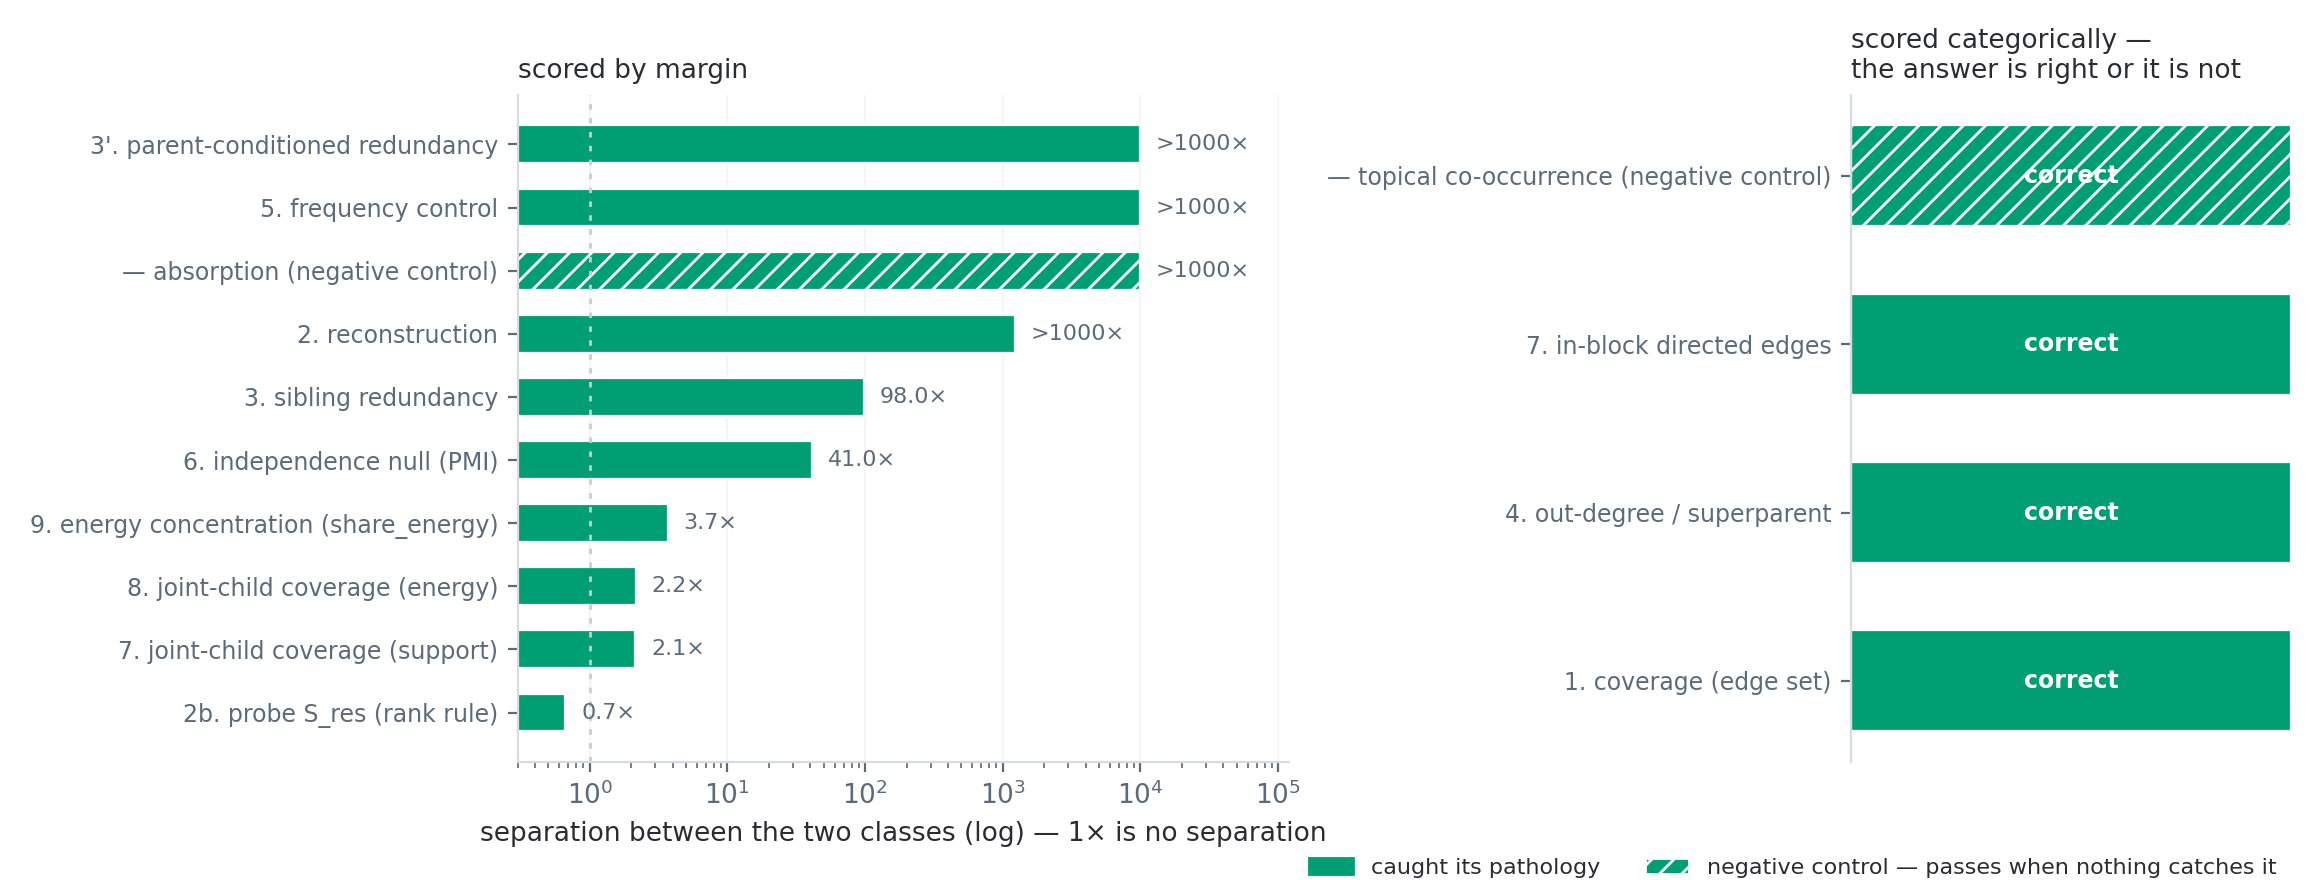
\includegraphics[width=\linewidth]{calibration_synthetic_toy_scorecard}
  \caption{%
    \textbf{Every metric scored against a known tree.}
    All 14 scorecard rows on a hand-built world with a known five-parent tree and six injected
    structures; 14 pass, across seeds 0--7, covering 21 of 21 metric functions. \emph{Left:}
    rows whose two classes separate by a ratio, on a log axis. \emph{Right:} rows scored
    categorically, where the recovered answer is either right or not. The two are kept apart
    because a categorical margin of $1.0$ means \emph{correct}, and on a ratio axis that would
    read as \emph{no separation at all}. The two hatched rows are negative controls, which
    pass when the battery does \emph{not} act: an absorbed child, whose true edge coverage can
    never propose because the child fires exactly where its parent is silent, and a
    shared-topic pair that clears coverage, reconstruction, the frequency control and the
    independence null. They turn the two open columns of the properties matrix into
    demonstrated limitations rather than asserted ones, and a regression makes them fail
    visibly.
  }
  \label{fig:calibration-synthetic-toy-scorecard}
\end{figure}

% [MAIN 2]
\begin{figure}[tbp]
  \centering
  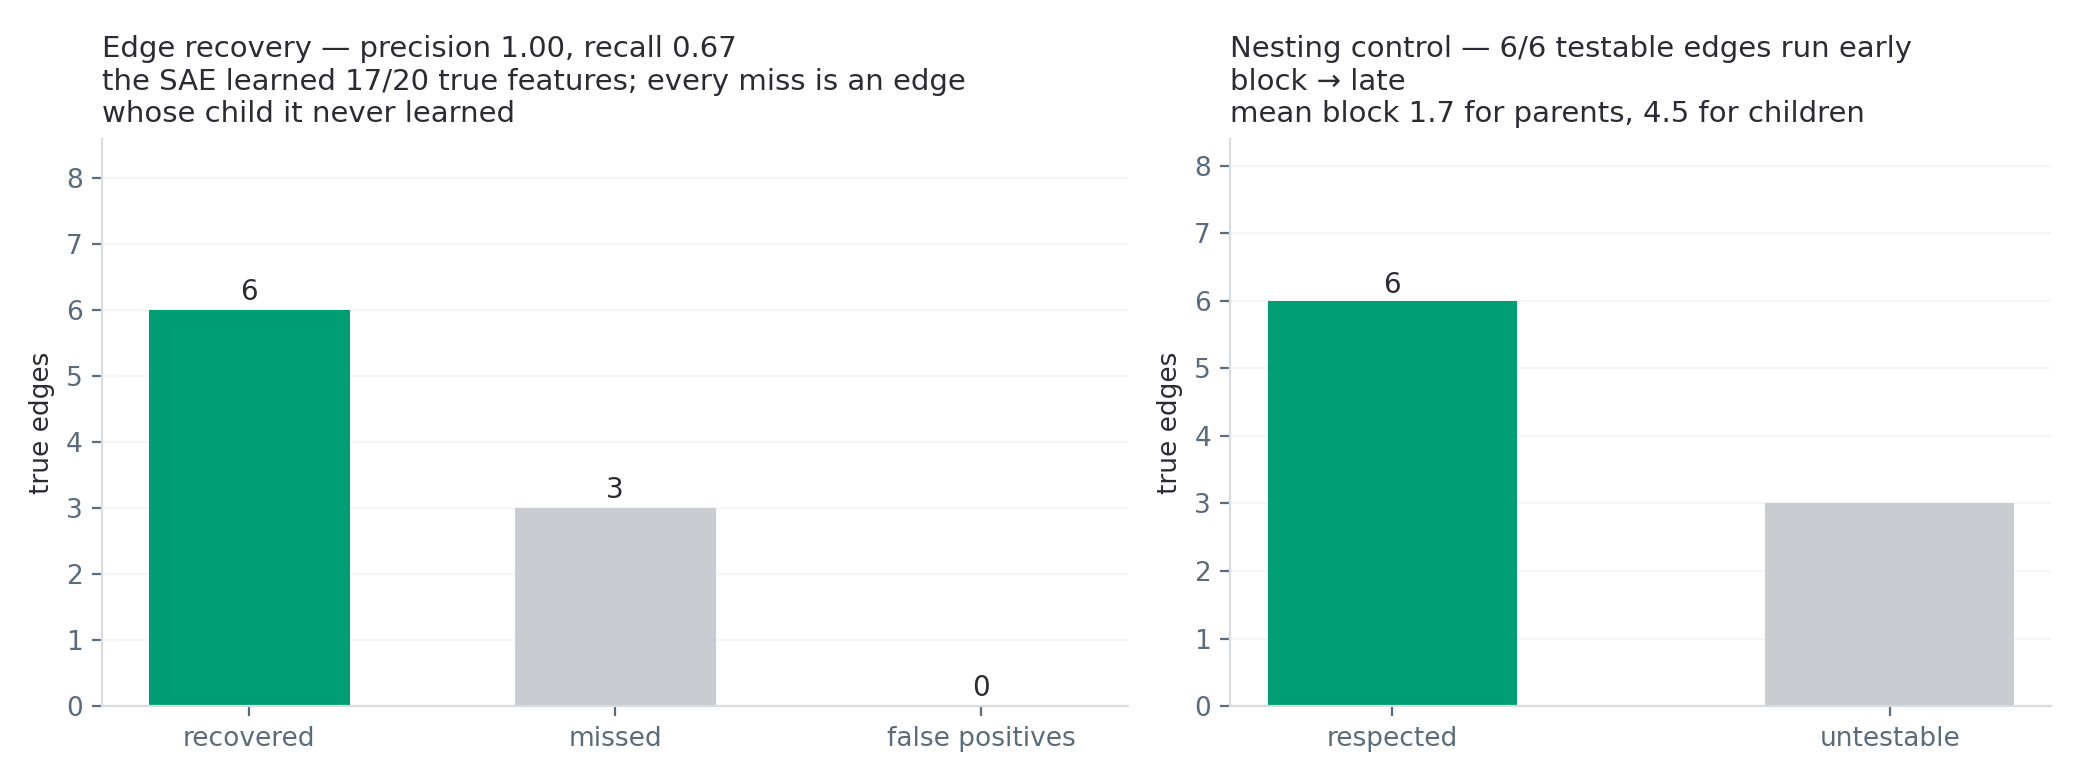
\includegraphics[width=\linewidth]{calibration_trained_toy_recovery}
  \caption{%
    \textbf{The same tree, after a real training run.}
    A Matryoshka SAE trained on the toy hierarchy, with the metrics run on the \emph{learned}
    latents rather than on constructed statistics. Precision 1.00, recall 0.67: 6 of 9 true
    edges recovered with 0 false positives, and every miss is an edge whose child the SAE
    never learned---it recovered 17 of 20 true features, which bounds recall from above.
    \emph{Right:} the lateral control, asking whether the Matryoshka nesting itself places a
    parent in an earlier block than its children. Beyond edge recovery, the parent-conditioned
    sibling metric reports 0.96 for one true parent against 0.00 and 0.00 for the others. The
    grammar declares every parent's children mutually exclusive, and they co-fire 0 times in
    200{,}000 draws; the latents that recovered them co-fire 27,592 times, and one of the two
    never fires alone. The SAE conflated two concepts the grammar keeps apart. This is a
    defect nobody injected, which the synthetic tier structurally cannot produce, and which
    the rest of the battery misses: both of that parent's edges are counted as recovered and
    precision stays $1.00$.
  }
  \label{fig:calibration-trained-toy-recovery}
\end{figure}

% -------------------------------------------------------------------------
% What the battery finds on gemma-2-2b
% -------------------------------------------------------------------------

% [MAIN 3]
\begin{figure}[tbp]
  \centering
  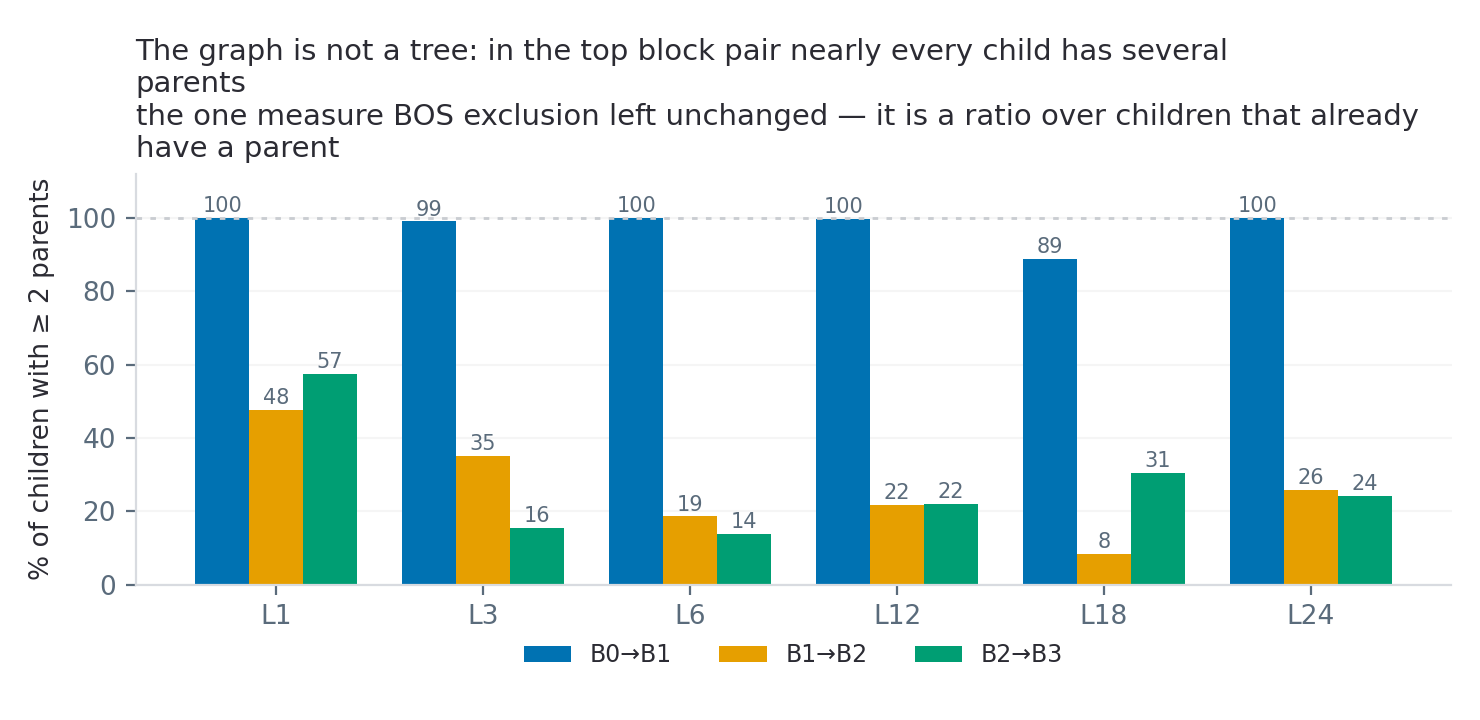
\includegraphics[width=\linewidth]{multiparenting_by_layer}
  \caption{%
    \textbf{The recovered graph is not a tree.}
    Percentage of child features with two or more parents, per block pair, across the five
    graded layers. In the top pair B0$\rightarrow$B1 the value is 100\% / 99\% / 100\% / 100\%
    / 89\% / 100\%---nearly every child in the second block is claimed by several first-block
    features, which no reading as a hierarchy survives. This is the only one of the project's
    four original claims that BOS exclusion left unchanged, because it is a ratio over
    children that already have a parent rather than a count of candidate edges, and so does
    not depend on the contaminated candidate set. Deeper pairs are much lower, on candidate
    sets that are also much smaller.
  }
  \label{fig:multiparenting-by-layer}
\end{figure}

% [MAIN 4]
\begin{figure}[tbp]
  \centering
  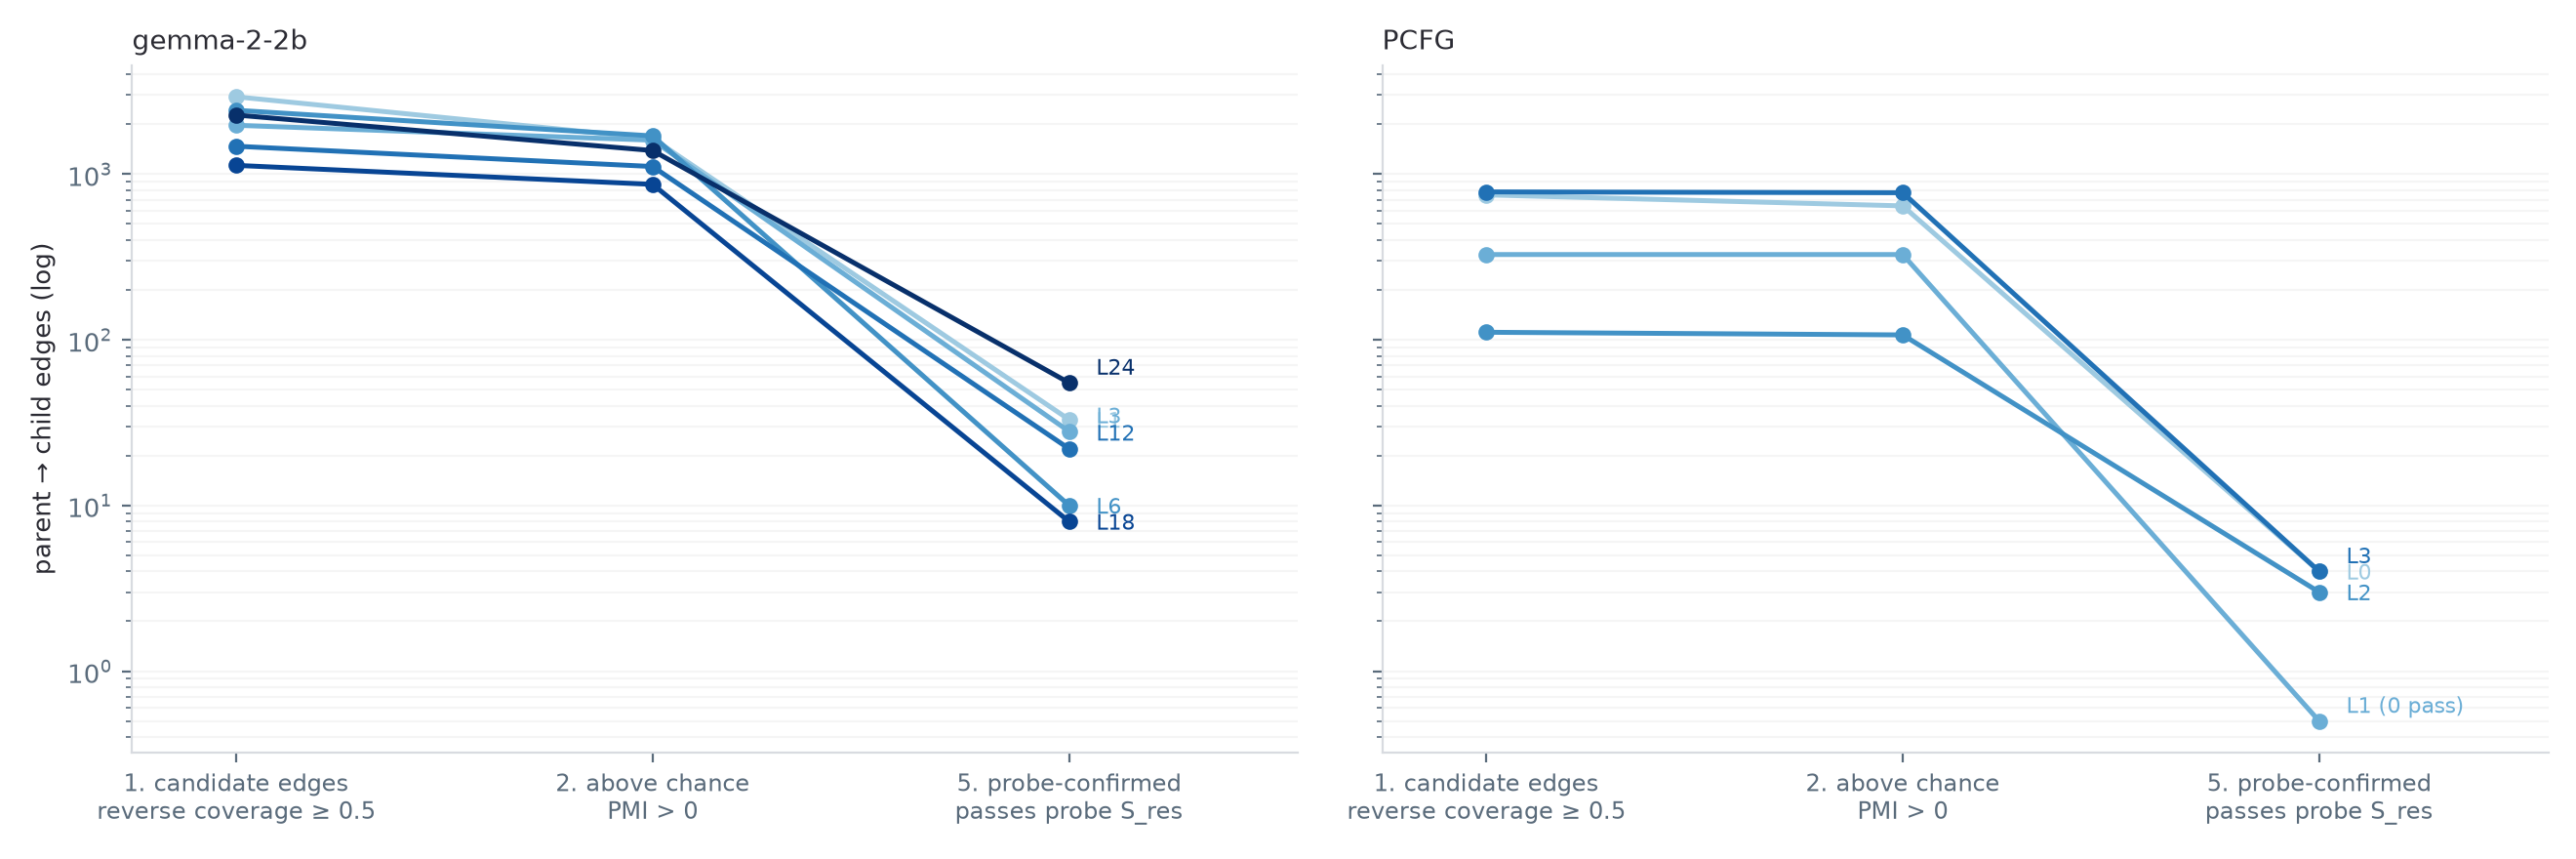
\includegraphics[width=\linewidth]{funnel_coverage_to_sres}
  \caption{%
    \textbf{Coverage proposes; the strict test disposes.}
    Block pair B0$\rightarrow$B1 of the layer-6 Matryoshka SAE on \texttt{gemma-2-2b}. Reverse
    coverage $R \geq 0.5$ with a joint-support guard admits 2,428 candidate edges. The
    reconstruction-ablation filter---drawn as a dashed reference rather than a funnel stage,
    because it is applied to all candidates in parallel and does not nest---passes 2,086 of
    them (86\%), so the cheap filter barely bites. Of the 1,700 edges reaching the probe-based
    $S_\mathrm{res}$ rank test, 10 pass (0.6\%). \textbf{Caveat:} stage~03 has been run on
    layer~6 only, so this ratio has a single layer behind it.
  }
  \label{fig:funnel-coverage-to-sres}
\end{figure}

% -------------------------------------------------------------------------
% The bottleneck-hijacking hypothesis, tested
% -------------------------------------------------------------------------

% [MAIN 5]
\begin{figure}[tbp]
  \centering
  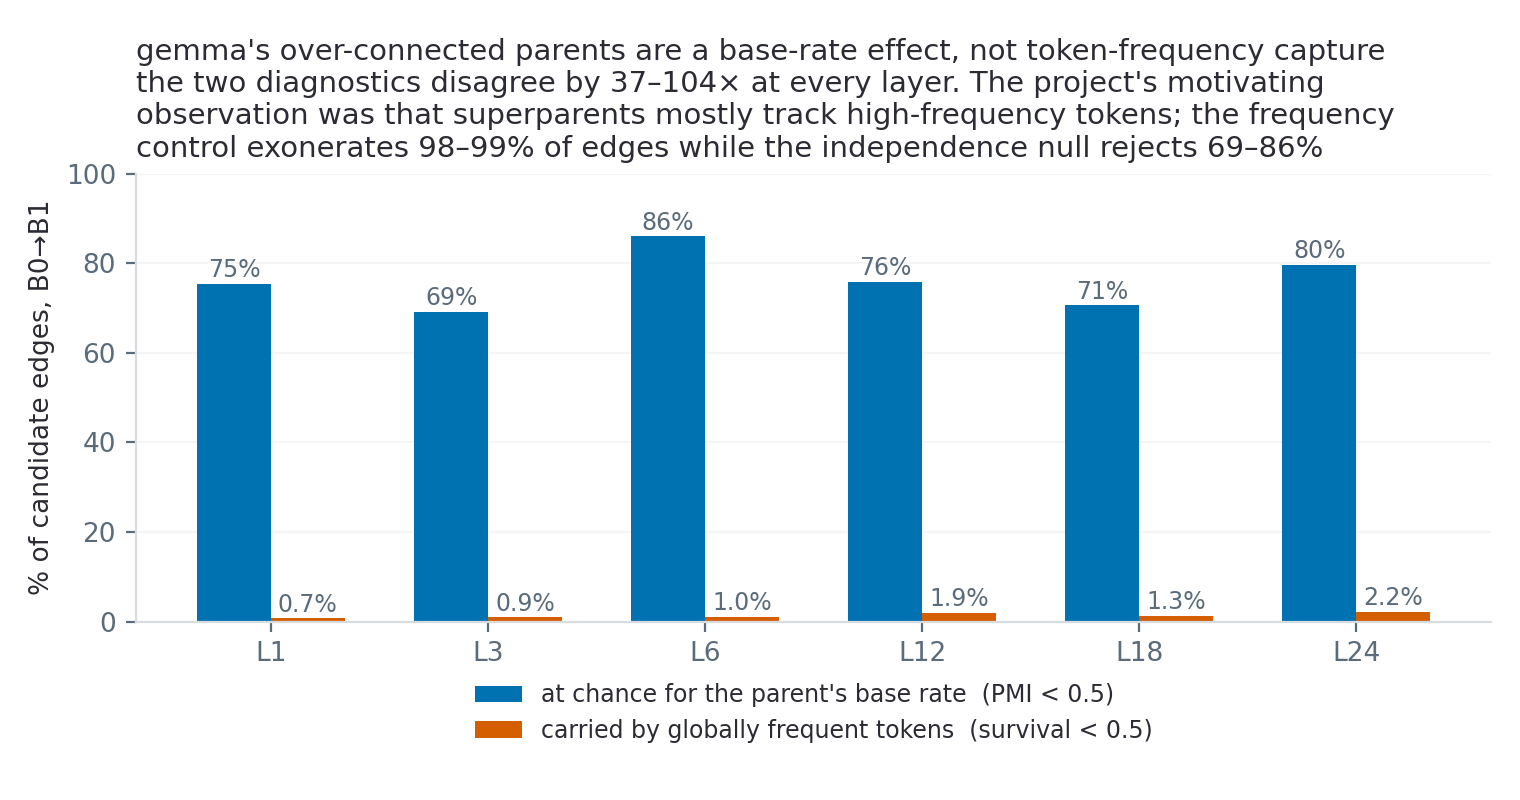
\includegraphics[width=\linewidth]{base_rate_vs_frequency_capture}
  \caption{%
    \textbf{The over-connection is a base-rate effect, not token-frequency capture.}
    Two per-edge diagnostics on the same candidate sets, B0$\rightarrow$B1. The independence
    null asks whether co-firing exceeds what the parent's own firing rate already forces, and
    rejects 69--86\% of edges. The token-frequency control asks whether the edge survives once
    globally frequent tokens are removed, and rejects 0.7--2.2\%. They disagree by
    37--104$\times$ at every layer. This tests the observation the bottleneck-hijacking
    hypothesis is built on---that the over-connected parents mostly track high-frequency
    tokens such as spaces, punctuation and \emph{the}---and does not support it: the frequency
    control exonerates 98--99\% of edges while the base-rate null rejects most of them.
  }
  \label{fig:base-rate-vs-frequency-capture}
\end{figure}

% [MAIN 6]
\begin{figure}[tbp]
  \centering
  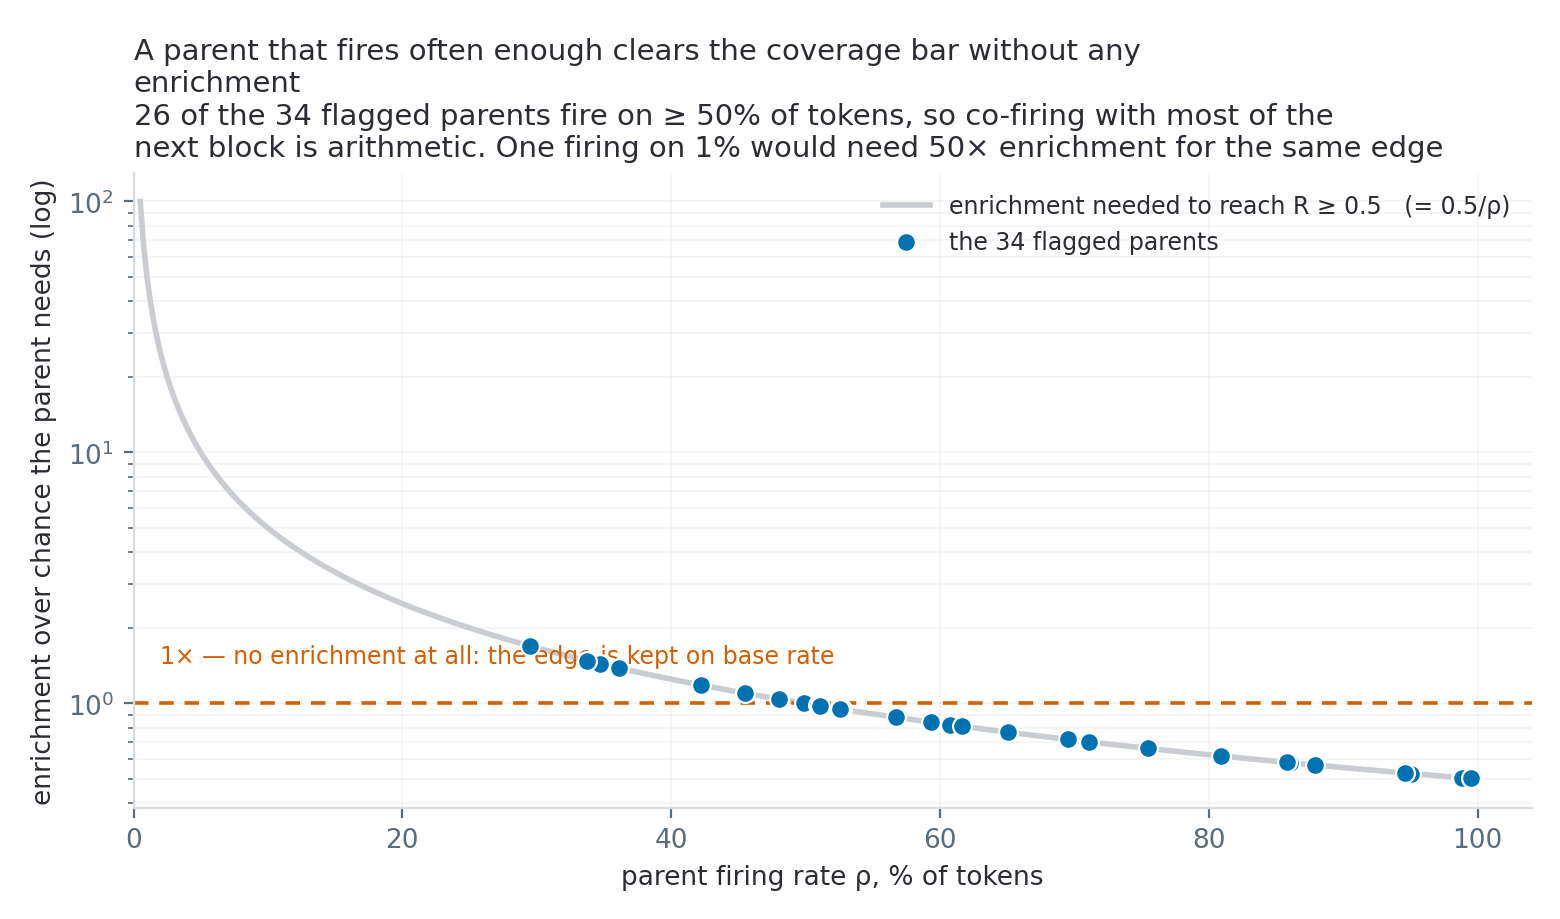
\includegraphics[width=\linewidth]{superparent_fanout_vs_firing}
  \caption{%
    \textbf{Why a parent that fires often enough clears the coverage bar for nothing.}
    An edge is kept when $P(\mathrm{parent} \mid \mathrm{child}) \geq \tau = 0.5$. Under
    independence that probability is simply the parent's firing rate $\rho$, so the enrichment
    a parent needs over chance is $\tau/\rho$, the grey curve. All 34 parents flagged as
    superparents, across five layers and every block pair, lie on it. 26 of them fire on at
    least 50\% of tokens and therefore clear the bar at $\leq 1\times$ enrichment---on base
    rate alone, with no association whatsoever between parent and child. A parent firing on
    1\% of tokens would need 50$\times$ enrichment for the same edge. This is the mechanism
    behind the previous figure.
  }
  \label{fig:superparent-fanout-vs-firing}
\end{figure}

% -------------------------------------------------------------------------
% What this says about metric batteries
% -------------------------------------------------------------------------

% [MAIN 7]
\begin{figure}[tbp]
  \centering
  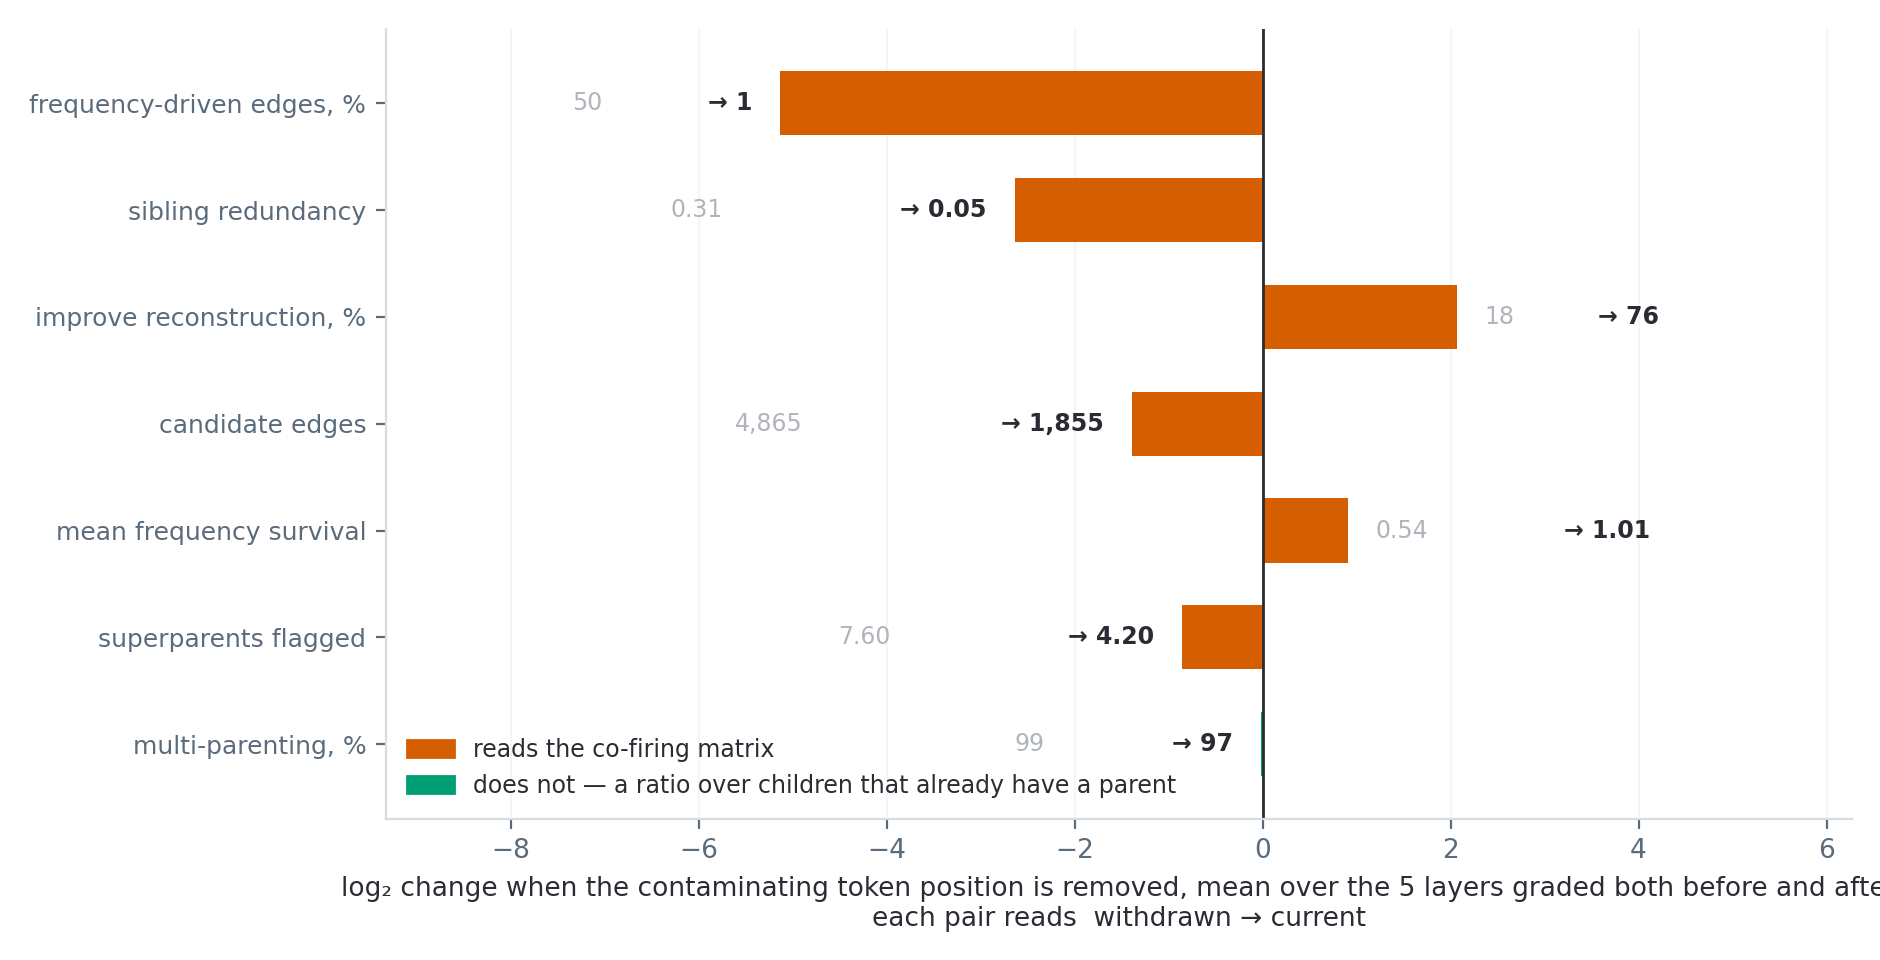
\includegraphics[width=\linewidth]{shared_input_moved_every_metric}
  \caption{%
    \textbf{Six metrics designed as independent detectors failed together.}
    Change in each metric, averaged over the five layers, when a single contaminating token
    position is excluded from the corpus. The beginning-of-sequence token is an attention sink
    on which effectively every feature fires; with 400 documents it handed every pair in the
    dictionary 400 joint firings against a support guard set at 30, so the guard admitted
    pairs that never co-occur anywhere else. Five of these six quantities are computed from
    that one co-firing matrix, and all five moved. The sixth, multi-parenting, is a ratio over
    children that already have a parent, does not read the matrix, and did not move. Agreement
    among detectors that share an input is far weaker evidence than the word \emph{battery}
    implies. The grey value in each pair is the withdrawn one, plotted to size the error and
    not as a result.
  }
  \label{fig:shared-input-moved-every-metric}
\end{figure}

% -------------------------------------------------------------------------
% Appendix
% -------------------------------------------------------------------------

% [APP 1]
\begin{figure}[tbp]
  \centering
  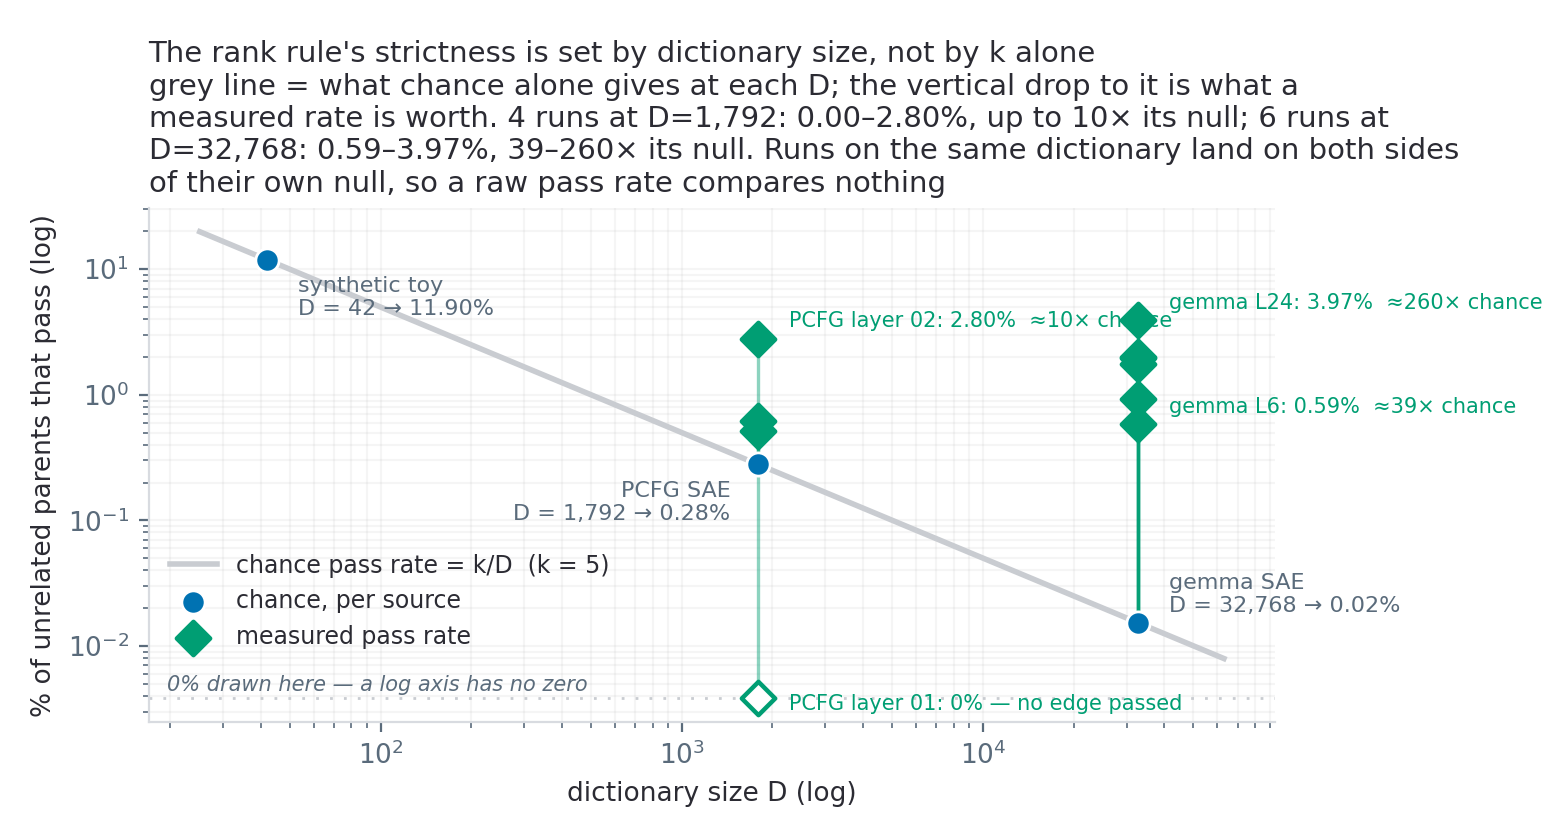
\includegraphics[width=\linewidth]{sres_null_rate_vs_dictionary_size}
  \caption{%
    \textbf{A top-$k$ rank rule is only as strict as the dictionary is large.}
    The $S_\mathrm{res}$ test passes an edge when both decoders fall within the top $k = 5$ of
    the probe's correlations over the whole dictionary. It is a geometry test, so an unrelated
    parent passes whenever chance places it there: the null rate is $k/D$, the grey line,
    which is $11.9\%$ on the 42-feature synthetic toy, $0.28\%$ on a 1{,}792-latent PCFG SAE
    and $0.015\%$ on gemma's 32{,}768. Each measured pass rate is drawn with a vertical drop
    to its own null, and that distance---not the rate---is what the measurement is worth. Two
    runs on the \emph{same} 1{,}792-latent dictionary land on opposite sides of their null,
    which is why a raw pass rate compares nothing across sources. A measured zero has no
    position on a logarithmic axis and is drawn at a marked floor rather than silently
    dropped.
  }
  \label{fig:sres-null-rate-vs-dictionary-size}
\end{figure}

% [APP 2]
\begin{figure}[tbp]
  \centering
  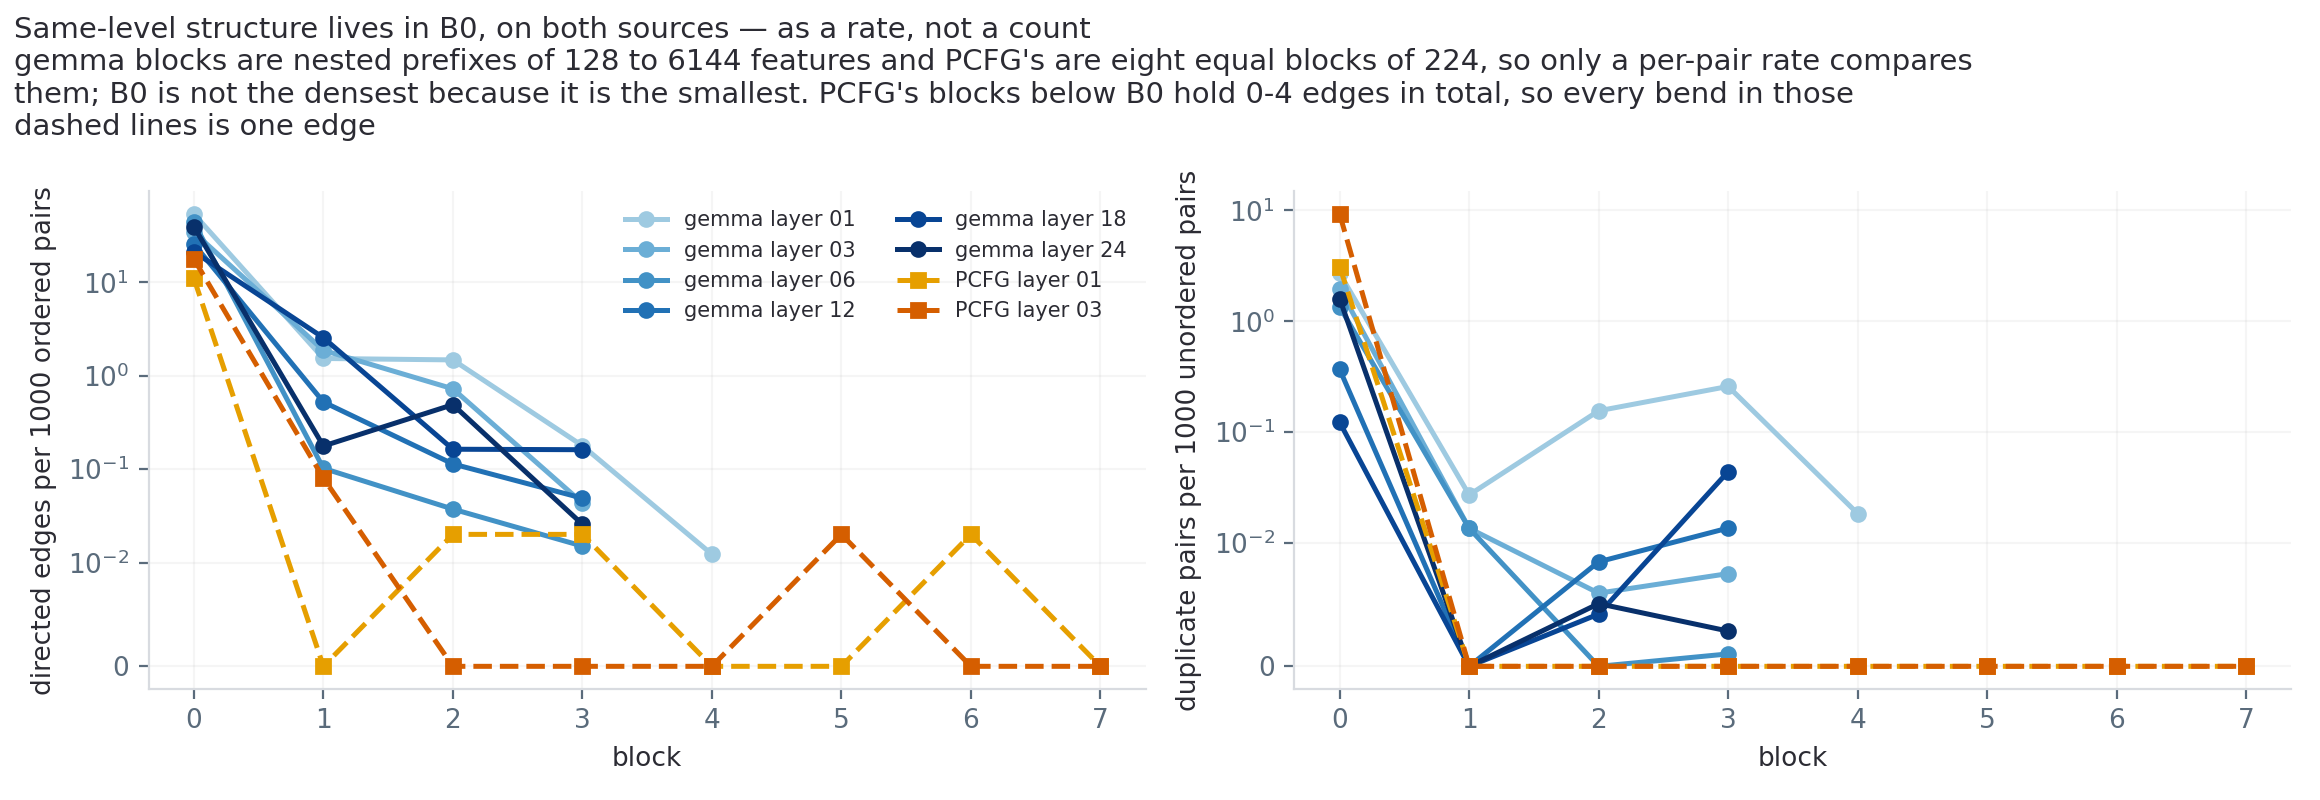
\includegraphics[width=\linewidth]{in_block_relations}
  \caption{%
    \textbf{Same-level structure lives in the outermost block.}
    Directed edges and co-extensive duplicates \emph{within} each block, where no block
    ordering fixes the direction and it must be derived from coverage asymmetry, across all 8
    graded runs. Reported as a rate per available pair rather than as a count: gemma's blocks
    are nested prefixes of 128 to 6{,}144 features, so the number of available pairs differs
    by a factor of 2{,}300 and raw counts invert the reading---the deepest block holds the
    most duplicate pairs and the fewest per pair. The concentration in B0 also holds on a PCFG
    SAE whose eight blocks are all 224 features, so it is not an artefact of B0 being small.
    What distinguishes B0 is being the outermost Matryoshka prefix: the one block trained to
    reconstruct on its own.
  }
  \label{fig:in-block-relations}
\end{figure}

% [APP 3]
\begin{figure}[tbp]
  \centering
  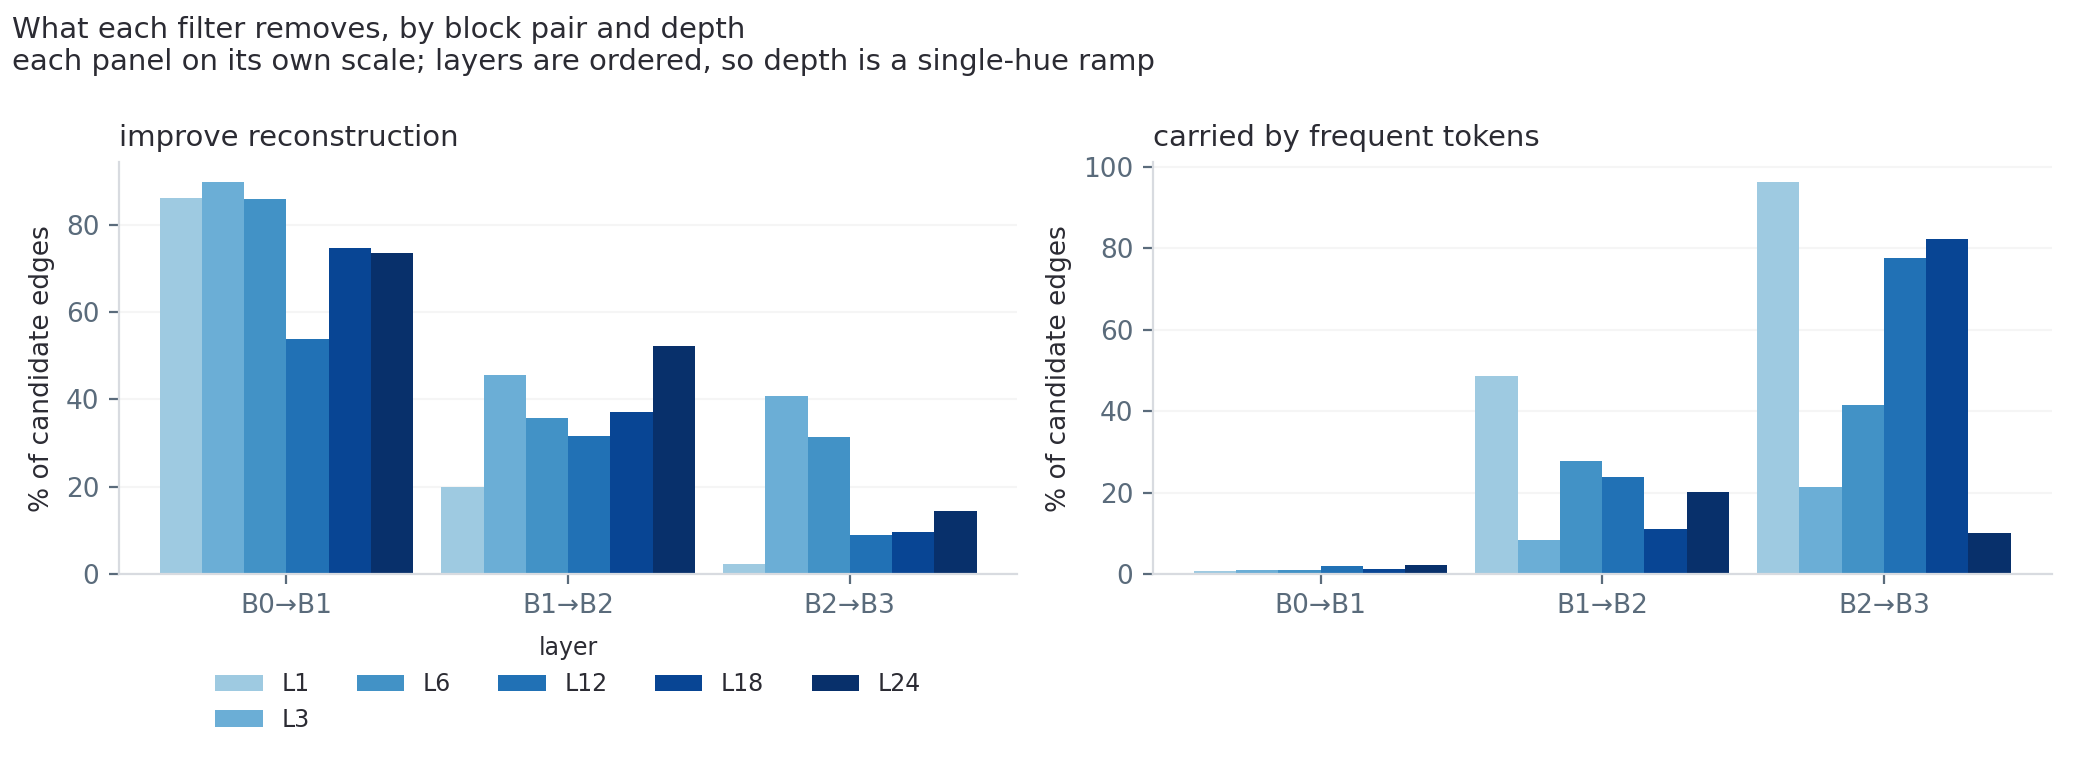
\includegraphics[width=\linewidth]{edge_survival_by_block_pair}
  \caption{%
    \textbf{What each filter removes, by block pair and by depth.}
    \emph{Left:} the share of candidate edges whose reconstruction improves when the parent is
    ablated. \emph{Right:} the share the token-frequency control judges to be carried by
    globally frequent tokens. Panels are on separate scales; layers are ordered, so depth is
    encoded as a single-hue ramp rather than as five categorical colours. The frequency
    control is nearly silent in the top block pair and rises sharply in the deeper ones, on
    candidate sets that are also far smaller there.
  }
  \label{fig:edge-survival-by-block-pair}
\end{figure}

% [APP 4]
\begin{figure}[tbp]
  \centering
  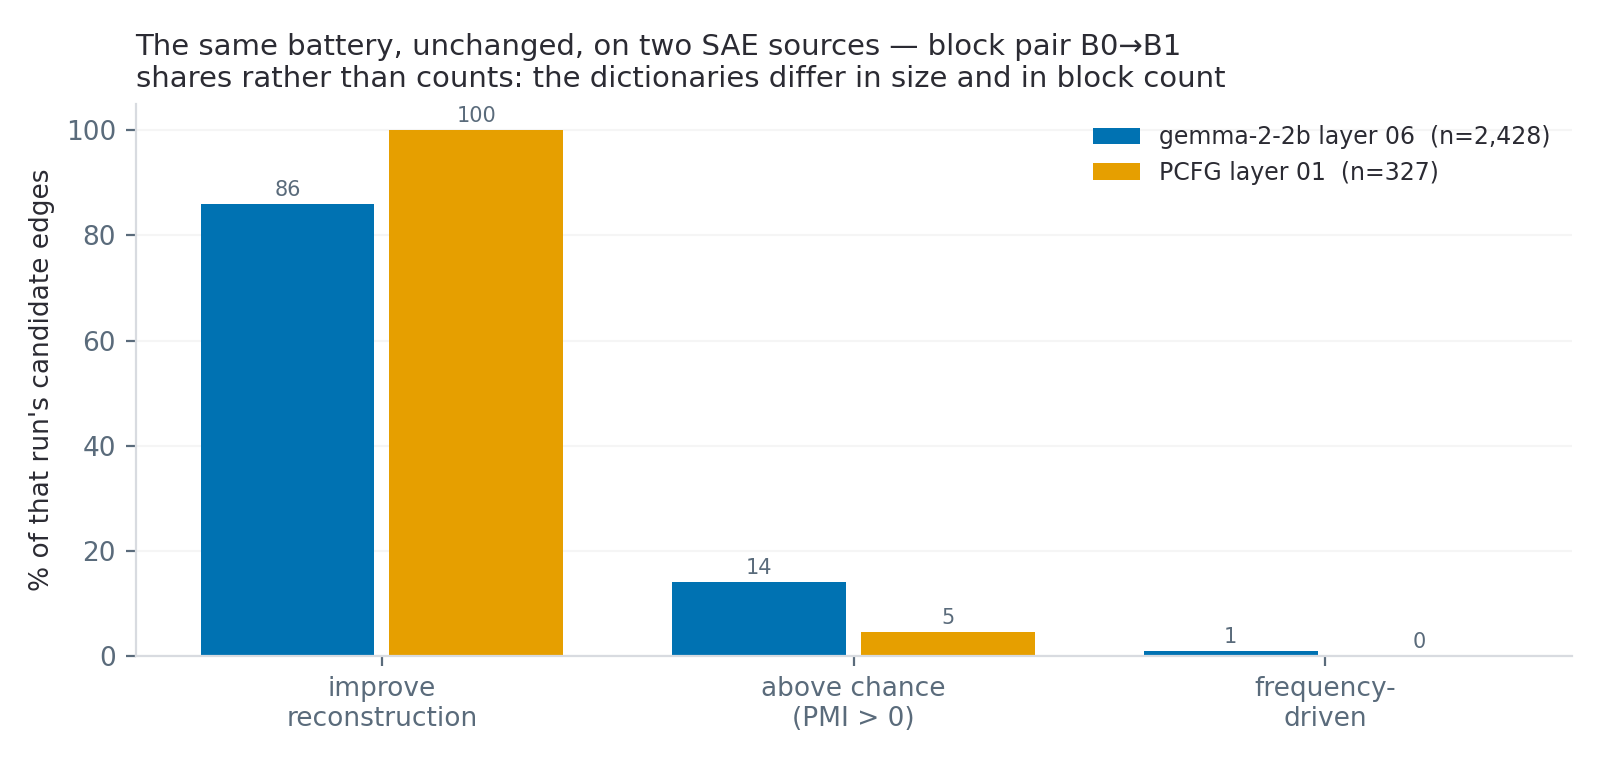
\includegraphics[width=\linewidth]{cross_source_funnel_shares}
  \caption{%
    \textbf{One unchanged battery across SAE sources.}
    The same metric code and the same global thresholds, applied to the released Matryoshka
    SAE on \texttt{gemma-2-2b} and to Matryoshka SAEs trained on a PCFG corpus. Reported as
    shares of each run's own candidate set, because the dictionaries differ in size and in
    block count and counts would not compare. Thresholds are deliberately not tuned per
    source: holding them fixed is what makes any cross-source comparison mean something. The
    reconstruction filter should be read with care on PCFG, where the weakest candidate edge
    sits $3.5\times$ above the threshold---the filter is inert there, and the surviving edges
    have passed coverage alone.
  }
  \label{fig:cross-source-funnel-shares}
\end{figure}

% [APP 5]
\begin{figure}[tbp]
  \centering
  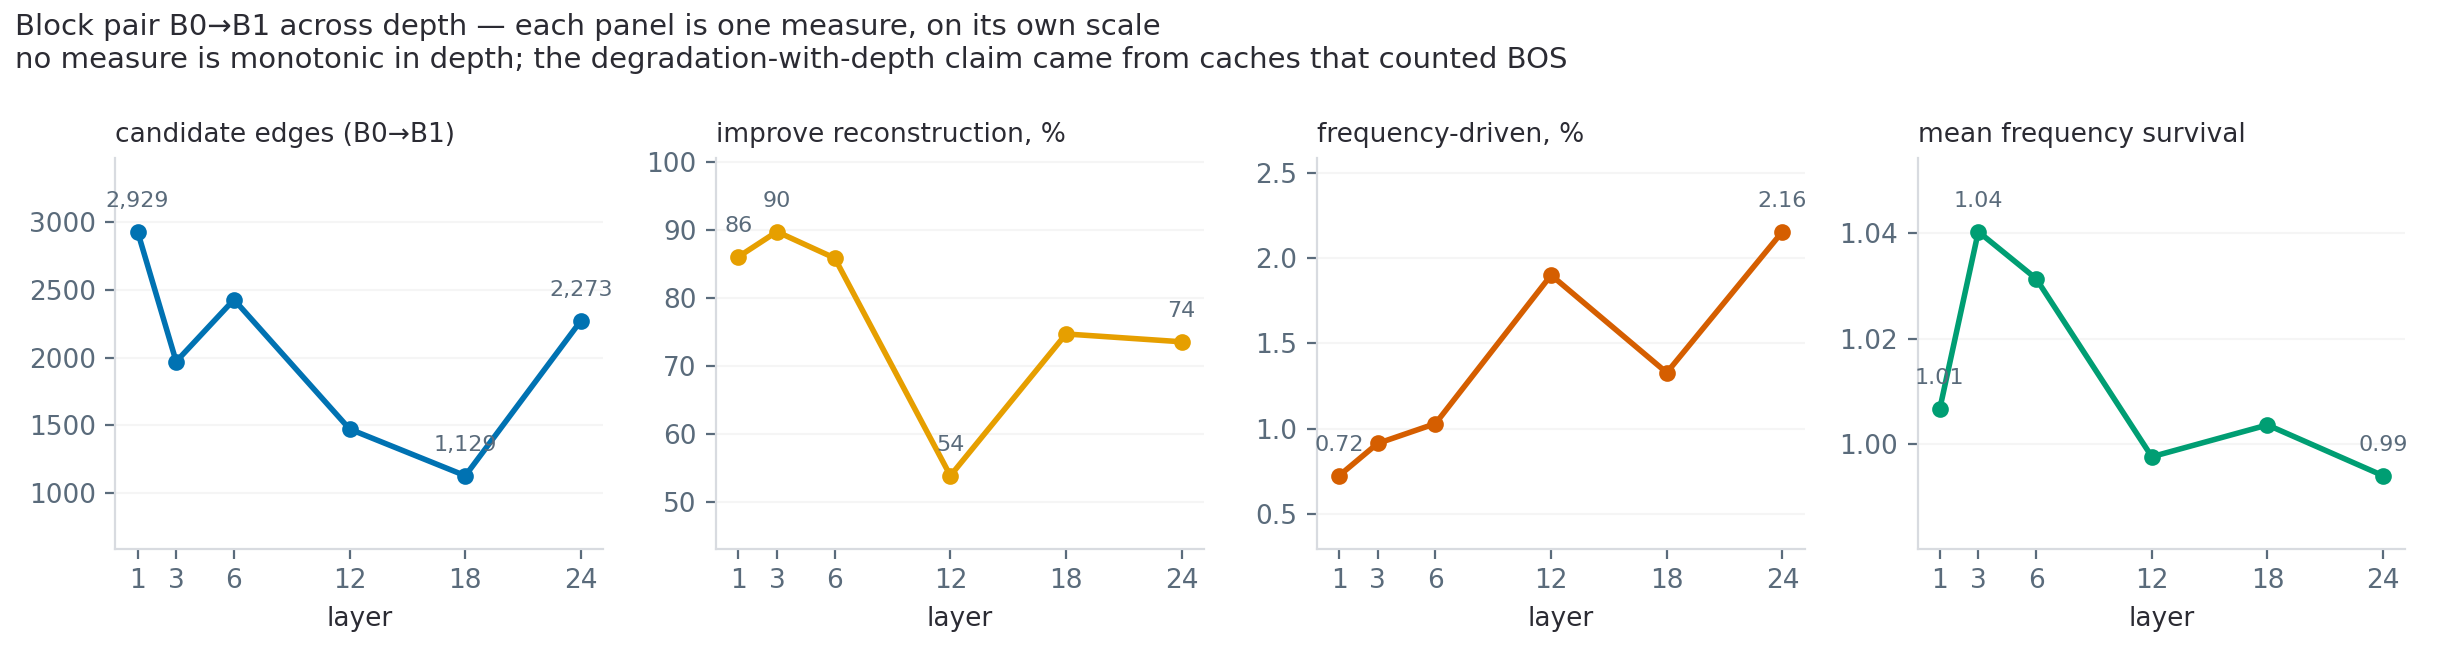
\includegraphics[width=\linewidth]{depth_profile_across_layers}
  \caption{%
    \textbf{No measure is monotonic in depth.}
    Four quantities for block pair B0$\rightarrow$B1 across the five graded layers, each on
    its own axis because they are not commensurable. The project previously reported that
    hierarchy quality degrades with depth. That claim came from caches in which the
    beginning-of-sequence position was counted, and it does not survive regeneration: the
    distinct-parent counts among survivors read 5, 7, 6, 7, 6. The figure is included because
    the withdrawal is itself a result about how easily a depth trend can be manufactured.
  }
  \label{fig:depth-profile-across-layers}
\end{figure}
